\subsection{Power}

Mobile devices employ dynamic voltage frequency scaling (DVFS),
  this results in power draw of the device being goverened by
  the operating frequency of the processor.
A typical model{\tt TODO:CITE Power tutor} of the power draw at time $t$ is

$$
P(t) = GPUV(GPUF(t)) + sum_{i=1}^{N} CPUV_n(CPUF_n(t))
$$

with $N$ begin the number of CPU cores, $GPUF(t)$ and $CPUF(t)$ are the operating frequencies at time $t$, and $GPUV(f)$ and $CPUV(f)$ are the power draws for the processors at the specified voltage.
Other terms, such as GPS, wireless, and other sensors, can be measured or modeled, but for this analysis we turn them off.

The of the issues with using a model are knowing the the power draw at the 
  frequency (which is not specified by the processor's manifacturer) and the method of reading
  the CPU and GPU counters is varies from device to device.
As a result, we use Qualcomm's Trepn tool {\tt TODO: CITE} to read the hardware
  counters.
Trepn, which is limited to Qualcomm based chipsets, reads internal processor
  counters as well as power rail information, both of which are not otherwise
  available programatically.
We set Trepn to read the counters every $100ms$ and measure the load and power
  usage seperatly to decrease the overhead of the profiler.



\begin{figure*}[ht]
  \centering
  \begin{subfigure}[b]{0.95\textwidth}
      \centering
      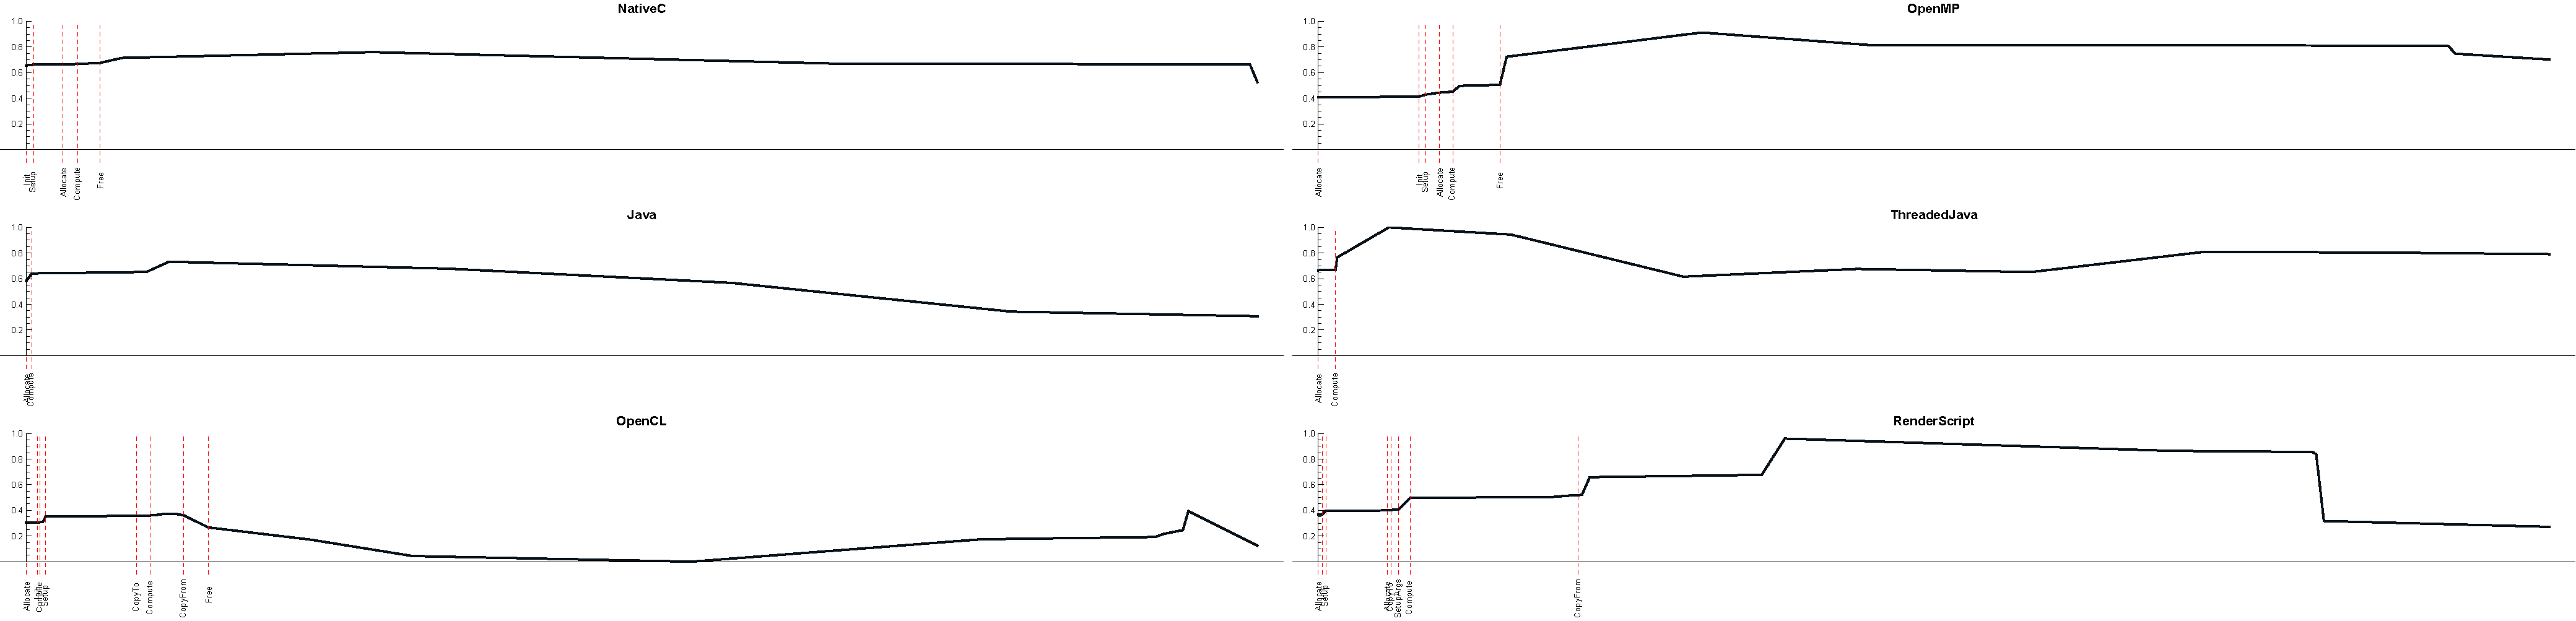
\includegraphics[width=\textwidth]{data/power_vectoradd_nexus5.pdf}
      \caption{VectorAdd}\label{fig:vectoradd}
  \end{subfigure}
  \begin{subfigure}[b]{0.95\textwidth}
      \centering
      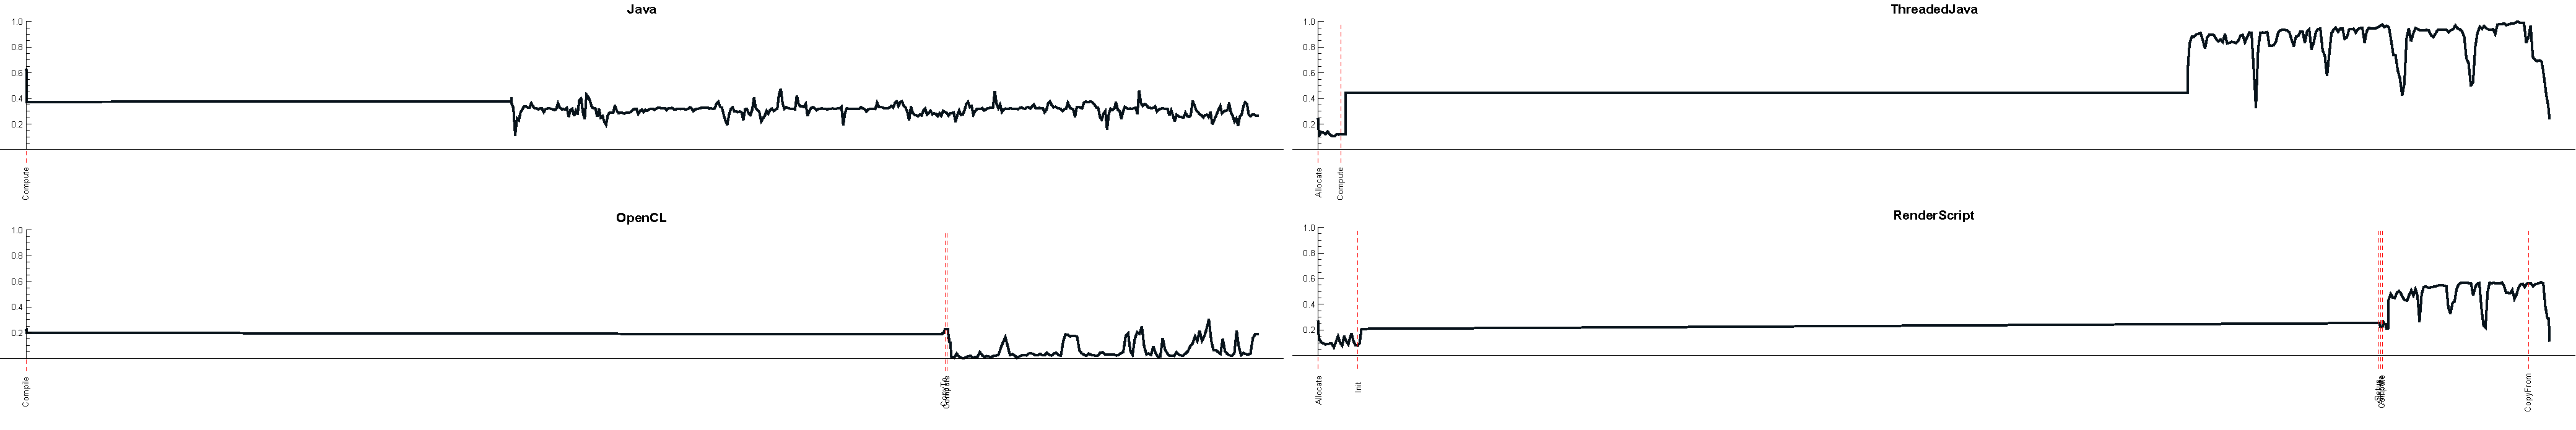
\includegraphics[width=\textwidth]{data/power_tpacf_nexus5.pdf}
      \caption{TPACF}
      \label{fig:TPACF}
  \end{subfigure}

  \begin{subfigure}[b]{0.95\textwidth}
      \centering
      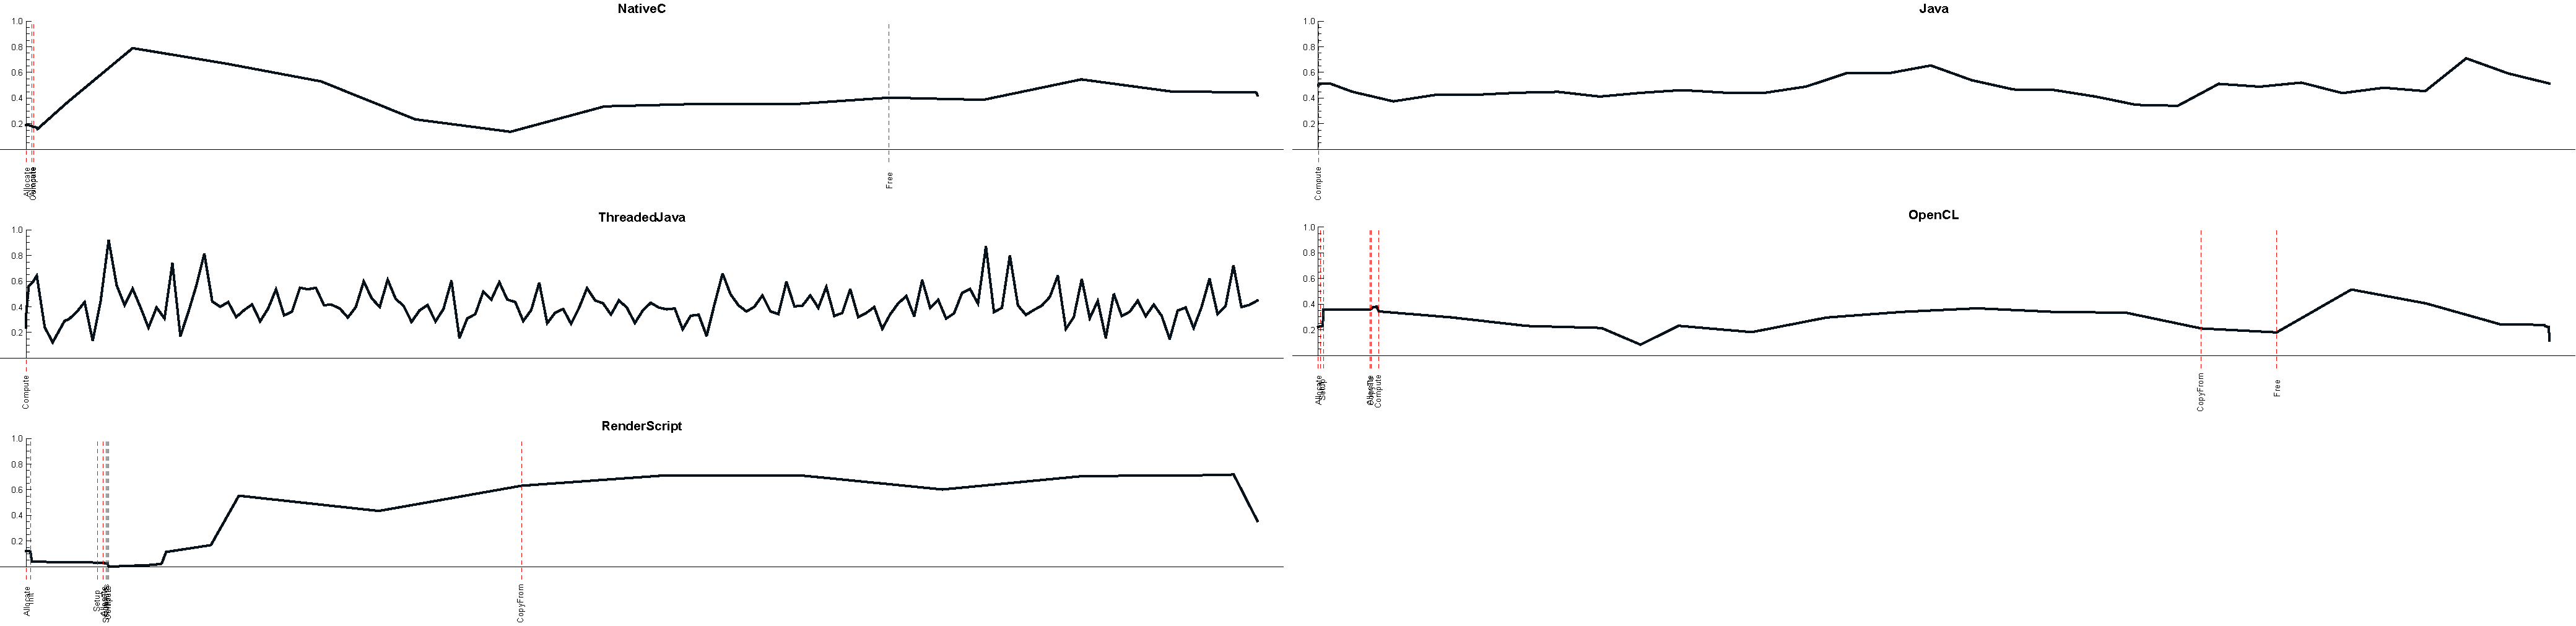
\includegraphics[width=\textwidth]{data/power_histogram_nexus5.pdf}
      \caption{Histo}\label{fig:histo}
  \end{subfigure}
  \begin{subfigure}[b]{0.95\textwidth}
      \centering
      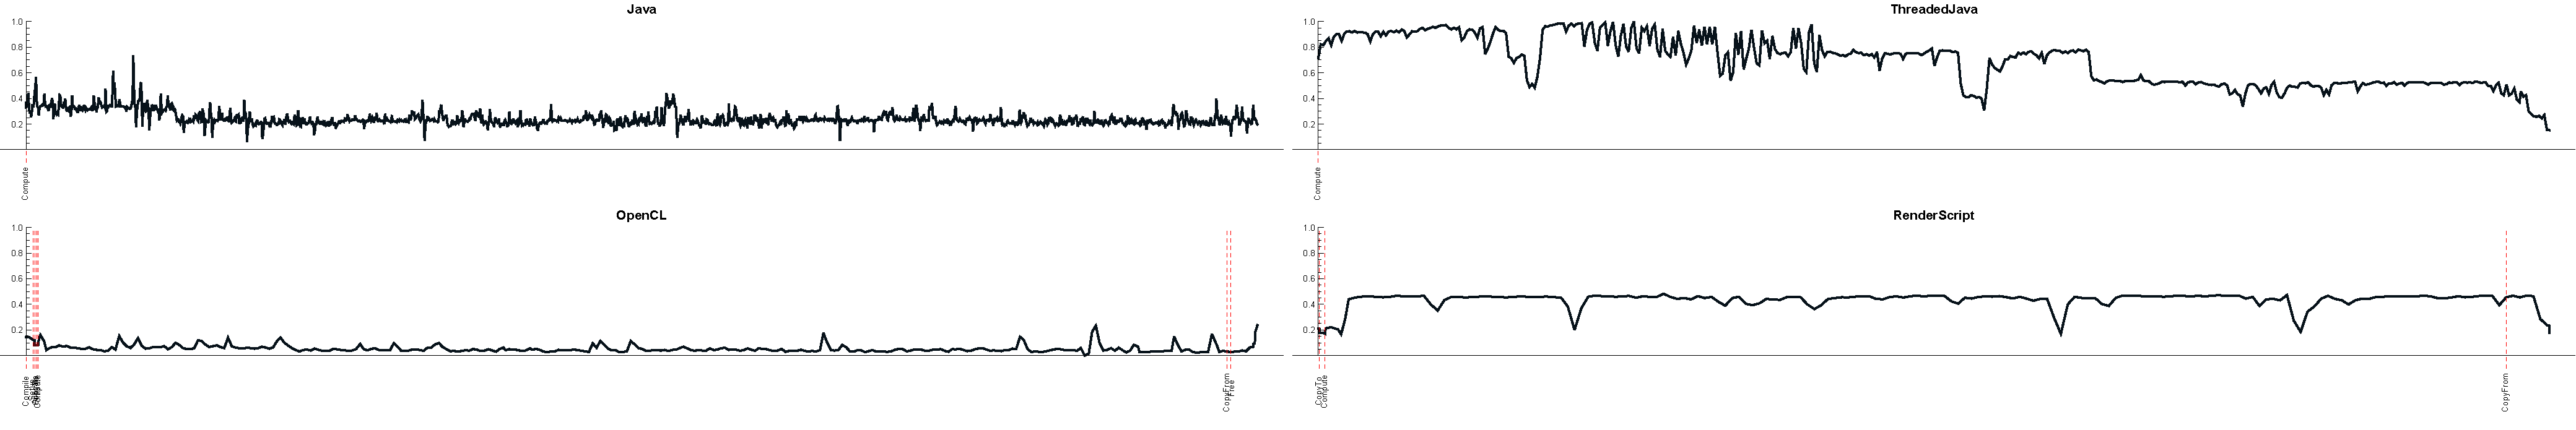
\includegraphics[width=\textwidth]{data/power_mriq_nexus5.pdf}
      \caption{MRIQ}
      \label{fig:MRIQ}
  \end{subfigure}

  \begin{subfigure}[b]{0.95\textwidth}
      \centering
      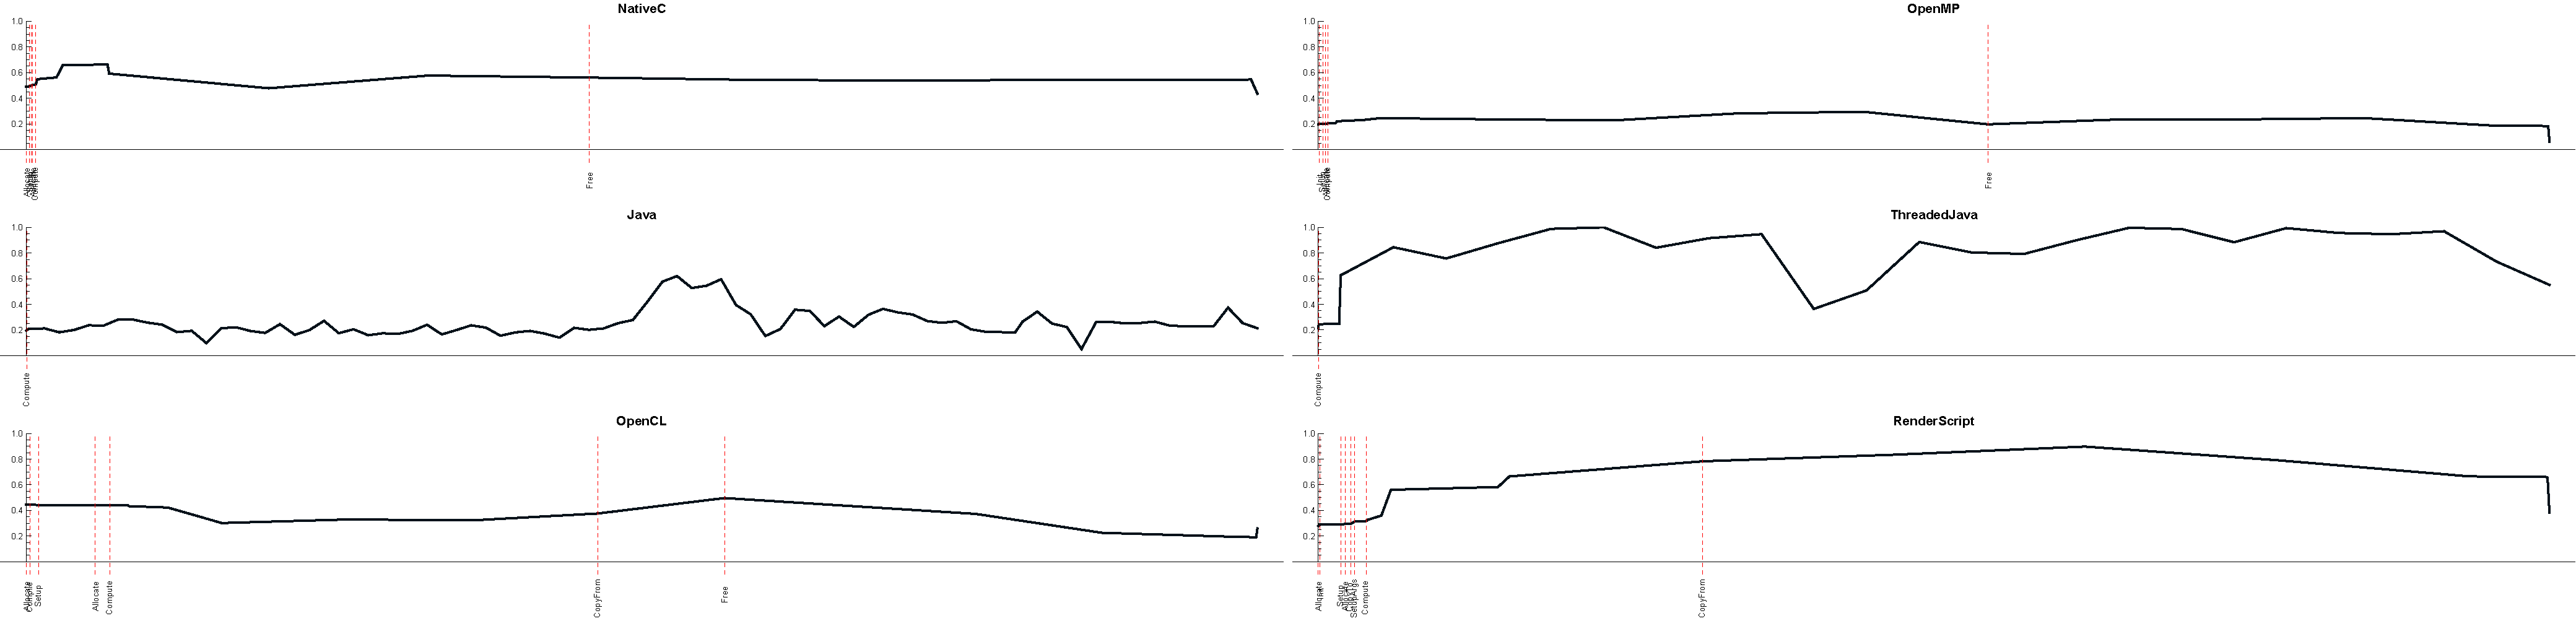
\includegraphics[width=\textwidth]{data/power_sgemm_nexus5.pdf}
      \caption{Sgemm}\label{fig:Sgemm}
  \end{subfigure}
  \begin{subfigure}[b]{0.95\textwidth}
      \centering
      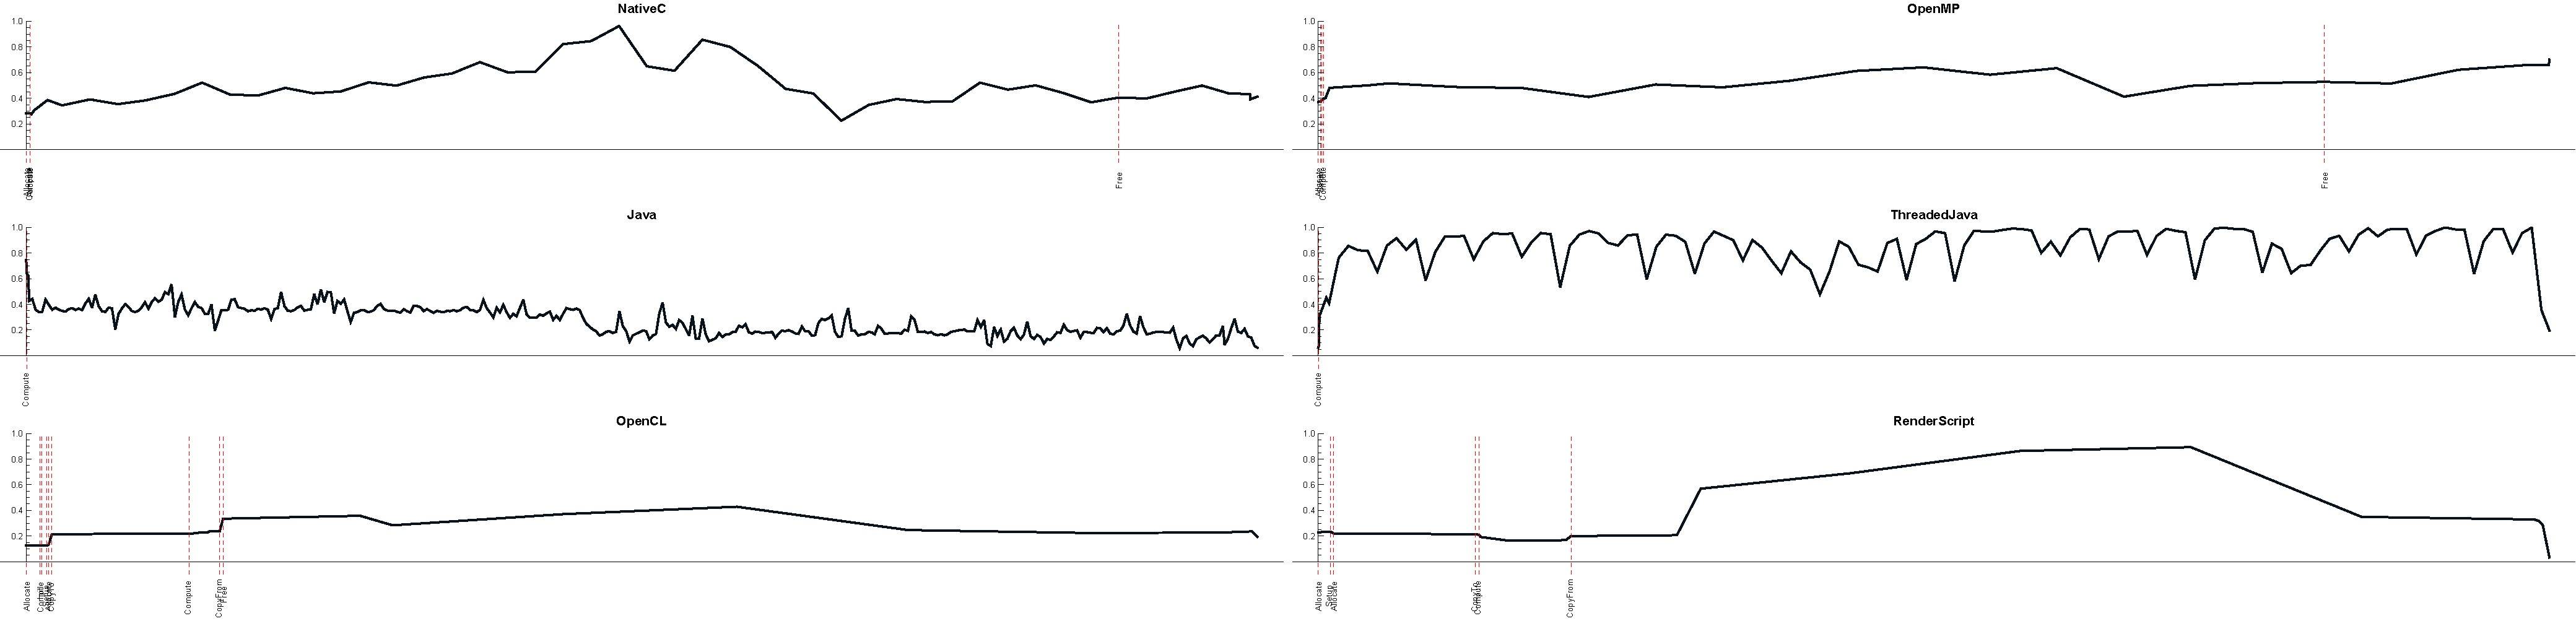
\includegraphics[width=\textwidth]{data/power_stencil_nexus5.pdf}
      \caption{Stencil}
      \label{fig:Stencil}
  \end{subfigure}

  \caption{Power Nexus 5}
\end{figure*}


\begin{figure*}[ht]
  \centering
  \begin{subfigure}[b]{0.95\textwidth}
      \centering
      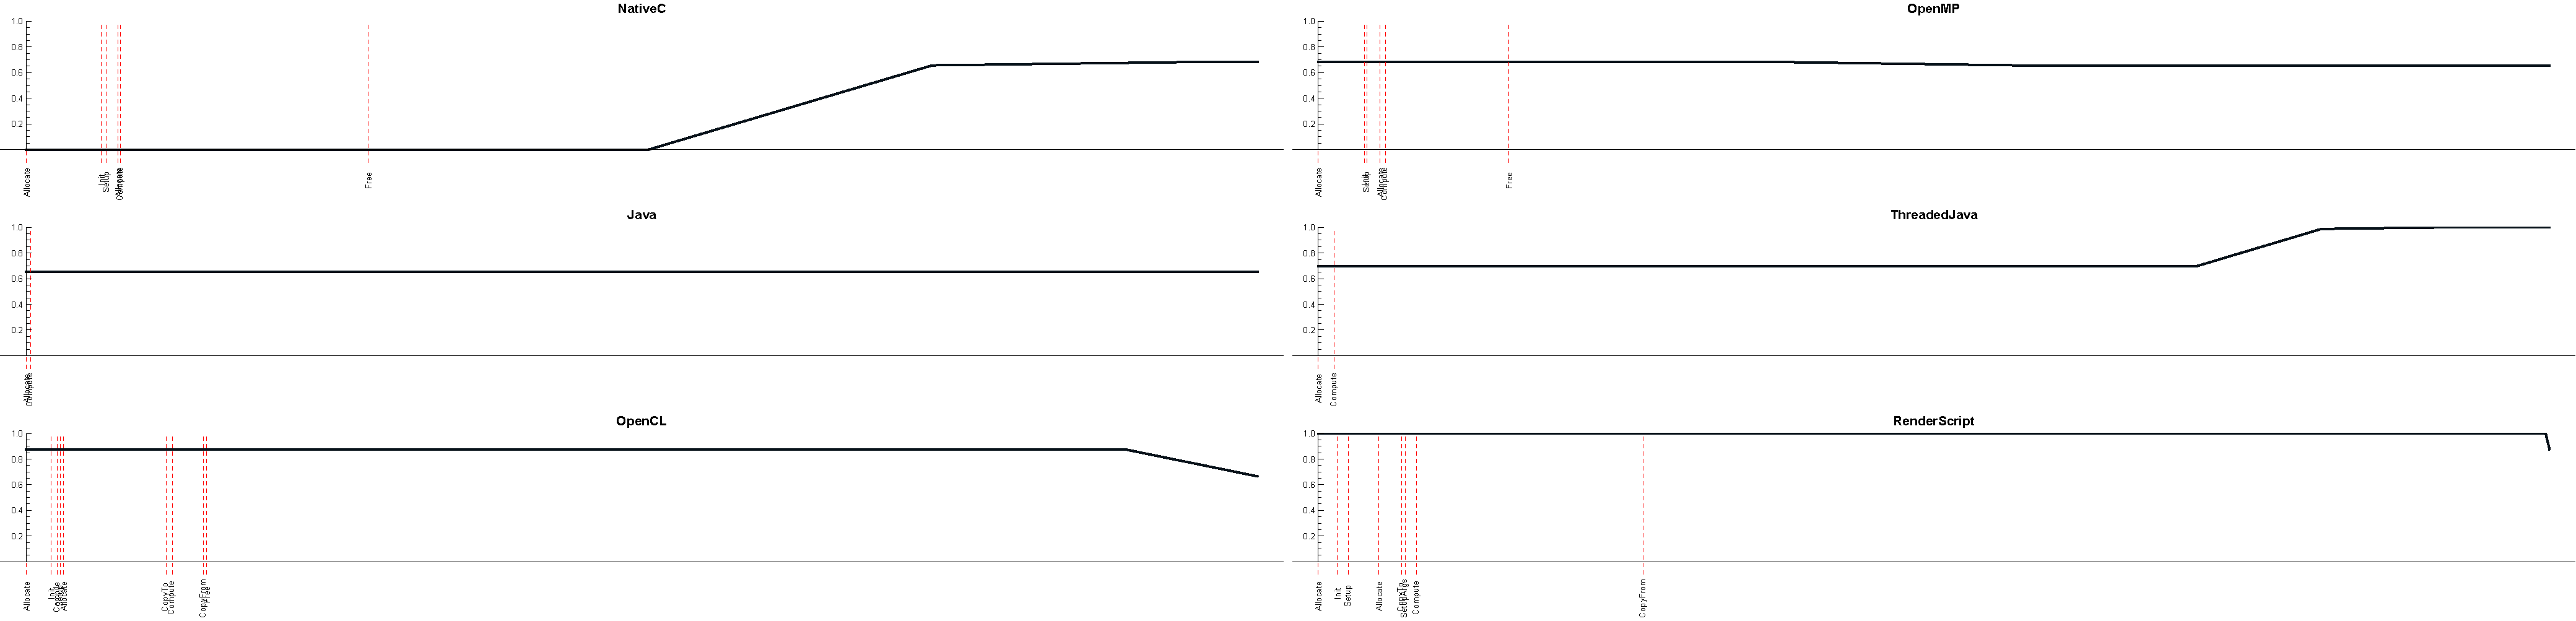
\includegraphics[width=\textwidth]{data/power_vectoradd_nexus7.pdf}
      \caption{VectorAdd}\label{fig:vectoradd}
  \end{subfigure}
  \begin{subfigure}[b]{0.95\textwidth}
      \centering
      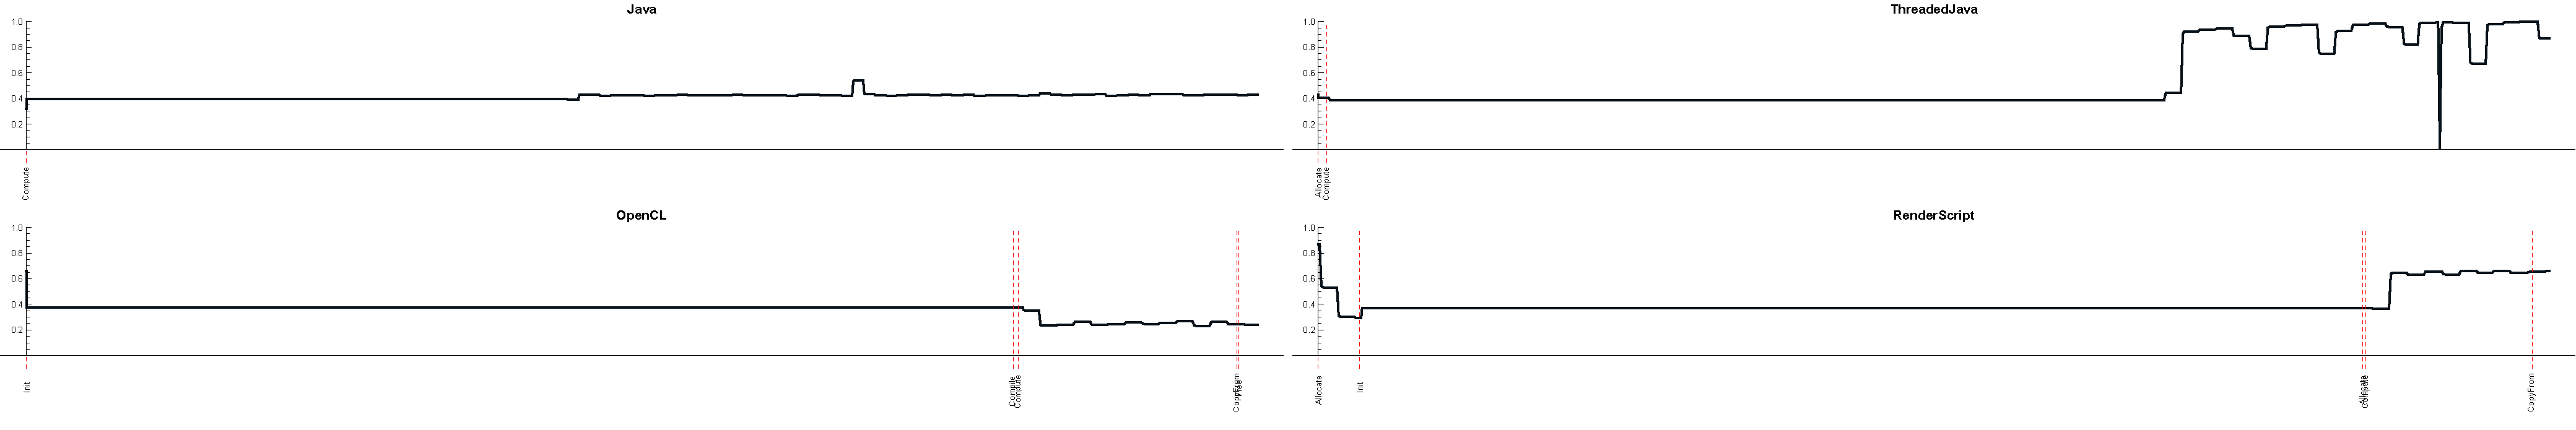
\includegraphics[width=\textwidth]{data/power_tpacf_nexus7.pdf}
      \caption{TPACF}
      \label{fig:TPACF}
  \end{subfigure}

  \begin{subfigure}[b]{0.95\textwidth}
      \centering
      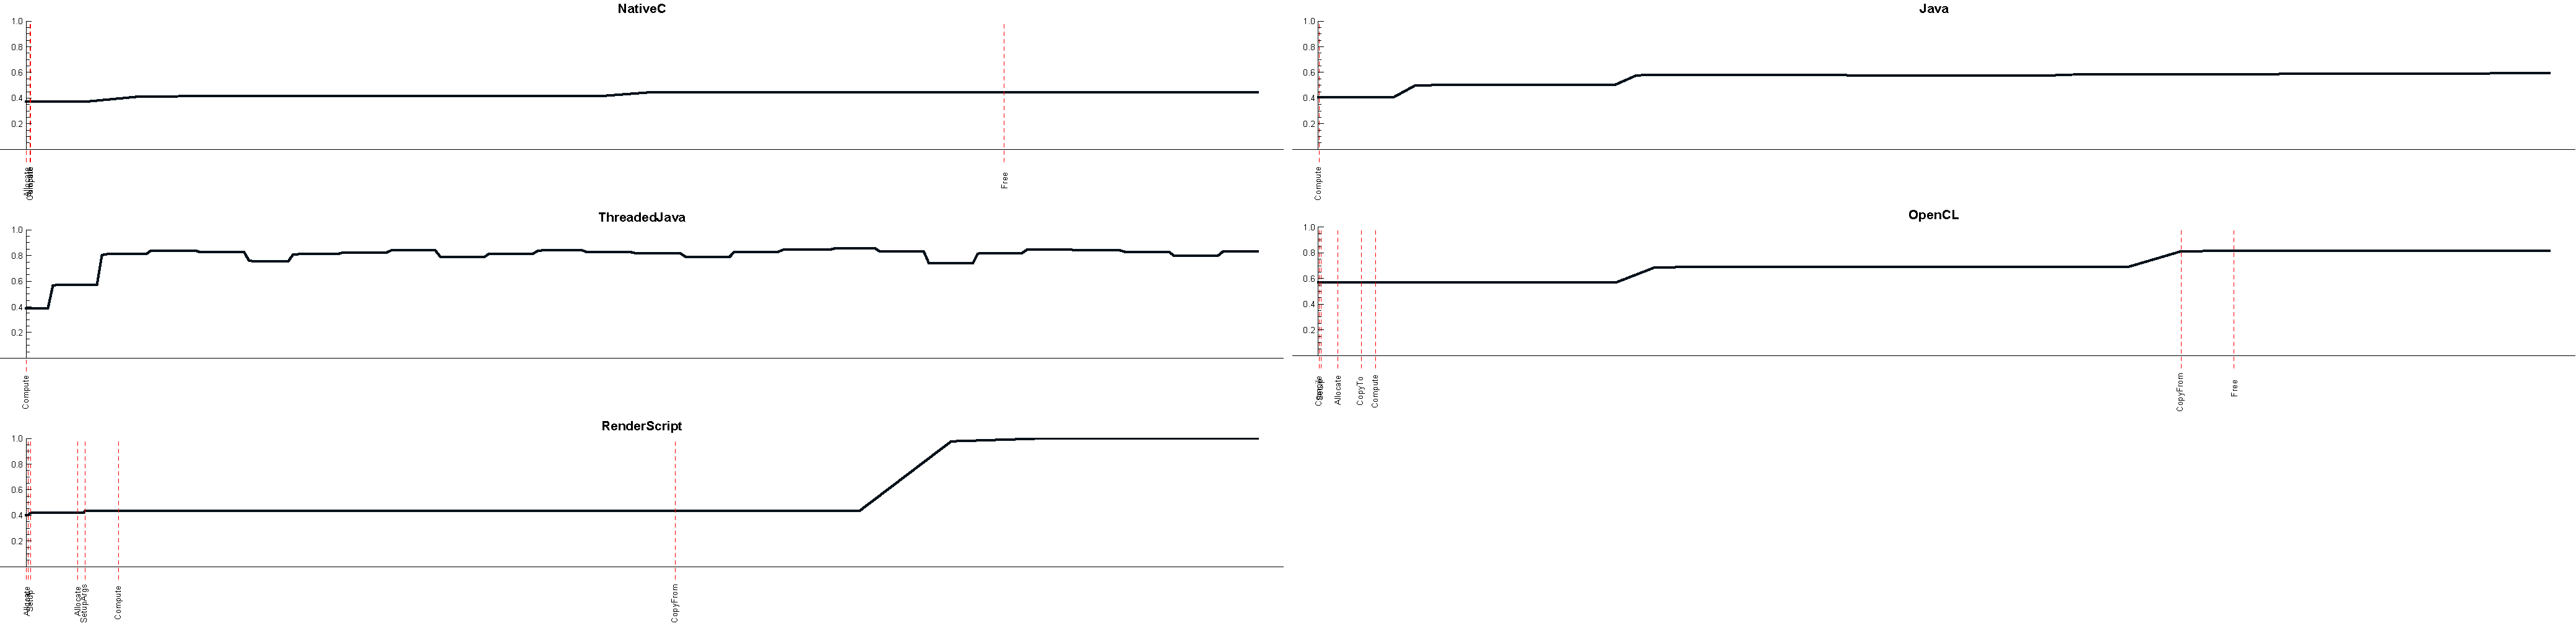
\includegraphics[width=\textwidth]{data/power_histogram_nexus7.pdf}
      \caption{Histo}\label{fig:histo}
  \end{subfigure}
  \begin{subfigure}[b]{0.95\textwidth}
      \centering
      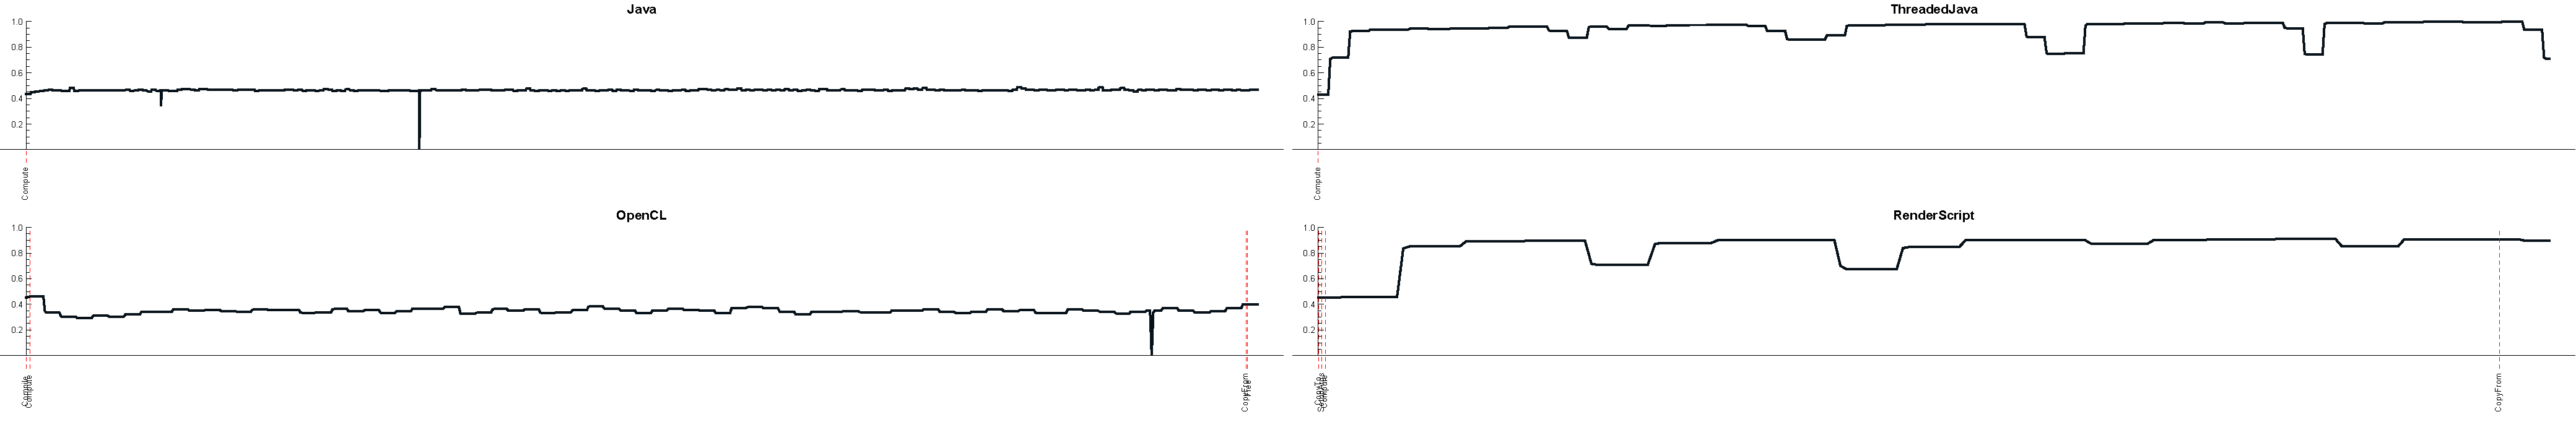
\includegraphics[width=\textwidth]{data/power_mriq_nexus7.pdf}
      \caption{MRIQ}
      \label{fig:MRIQ}
  \end{subfigure}

  \begin{subfigure}[b]{0.95\textwidth}
      \centering
      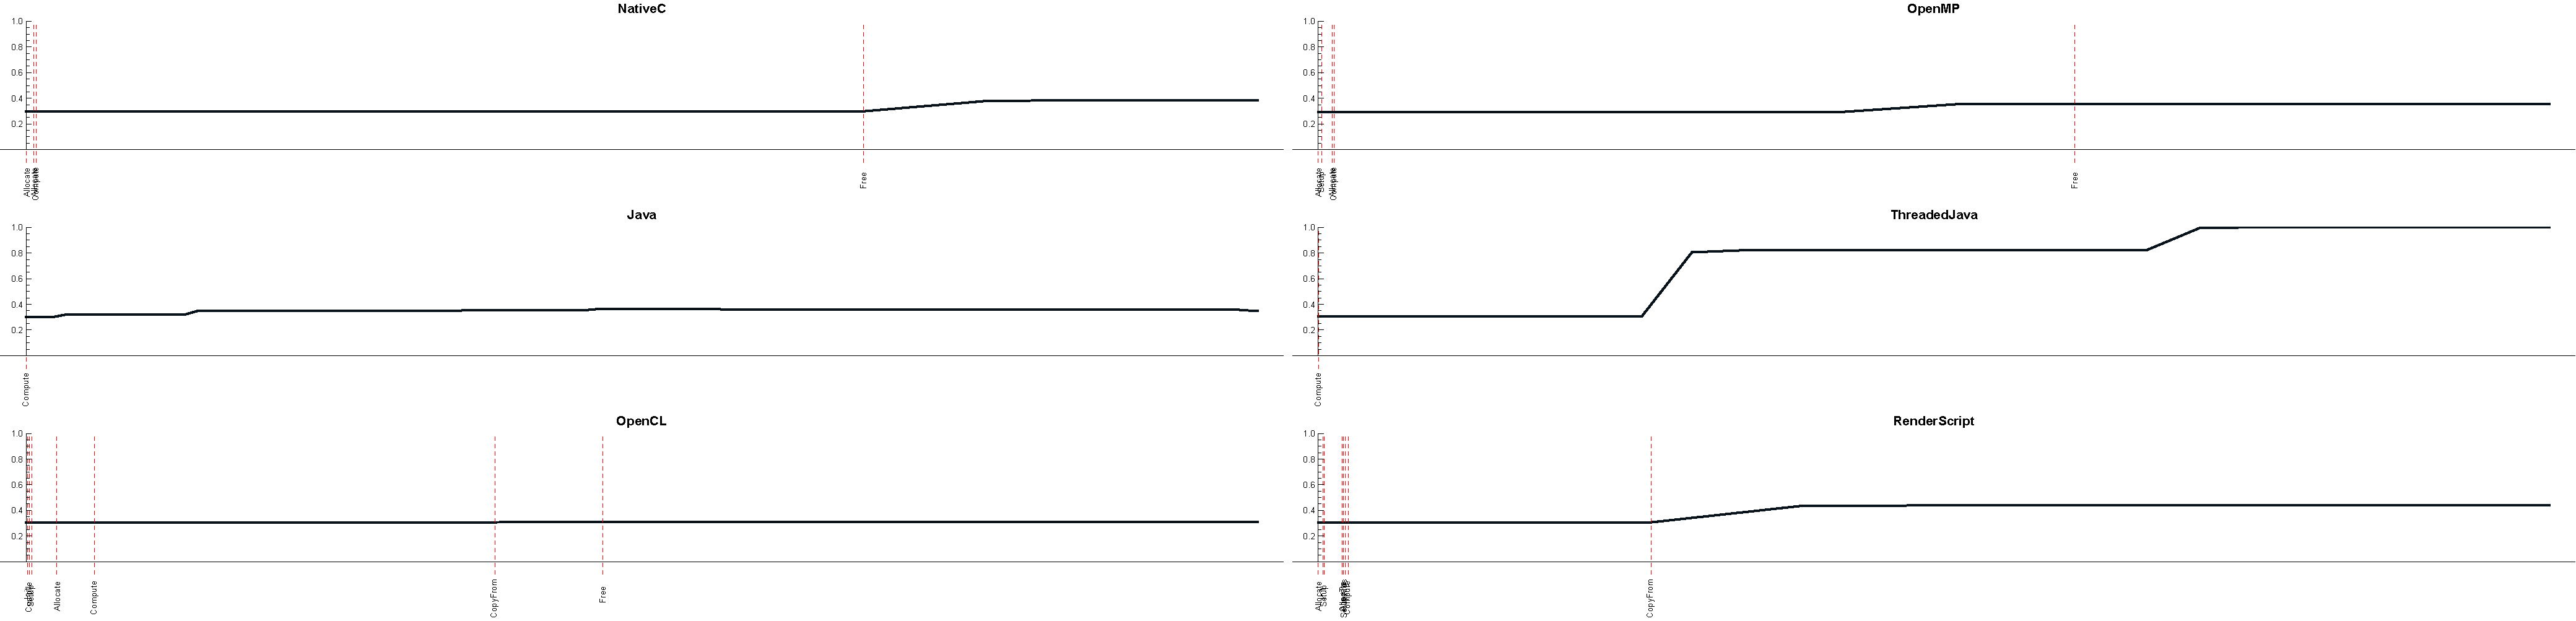
\includegraphics[width=\textwidth]{data/power_sgemm_nexus7.pdf}
      \caption{Sgemm}\label{fig:Sgemm}
  \end{subfigure}
  \begin{subfigure}[b]{0.95\textwidth}
      \centering
      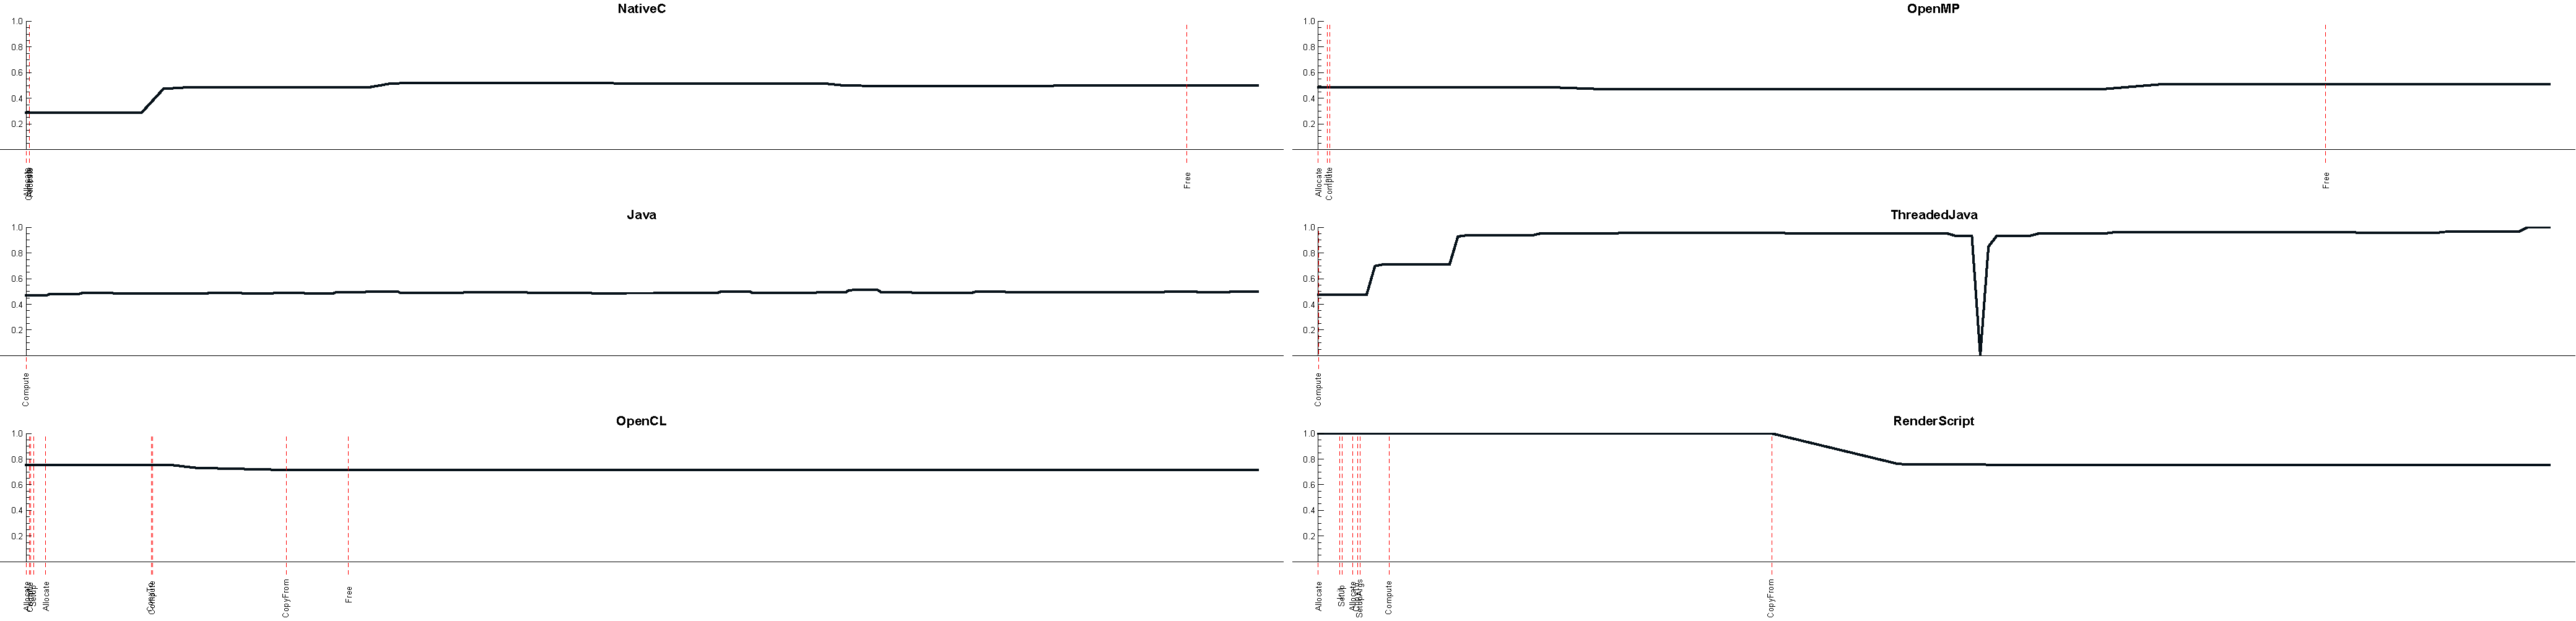
\includegraphics[width=\textwidth]{data/power_stencil_nexus7.pdf}
      \caption{Stencil}
      \label{fig:Stencil}
  \end{subfigure}

\caption{Power Nexus 7}
\end{figure*}



\begin{figure*}[ht]
  \begin{subfigure}[b]{0.5\textwidth}
      \centering
      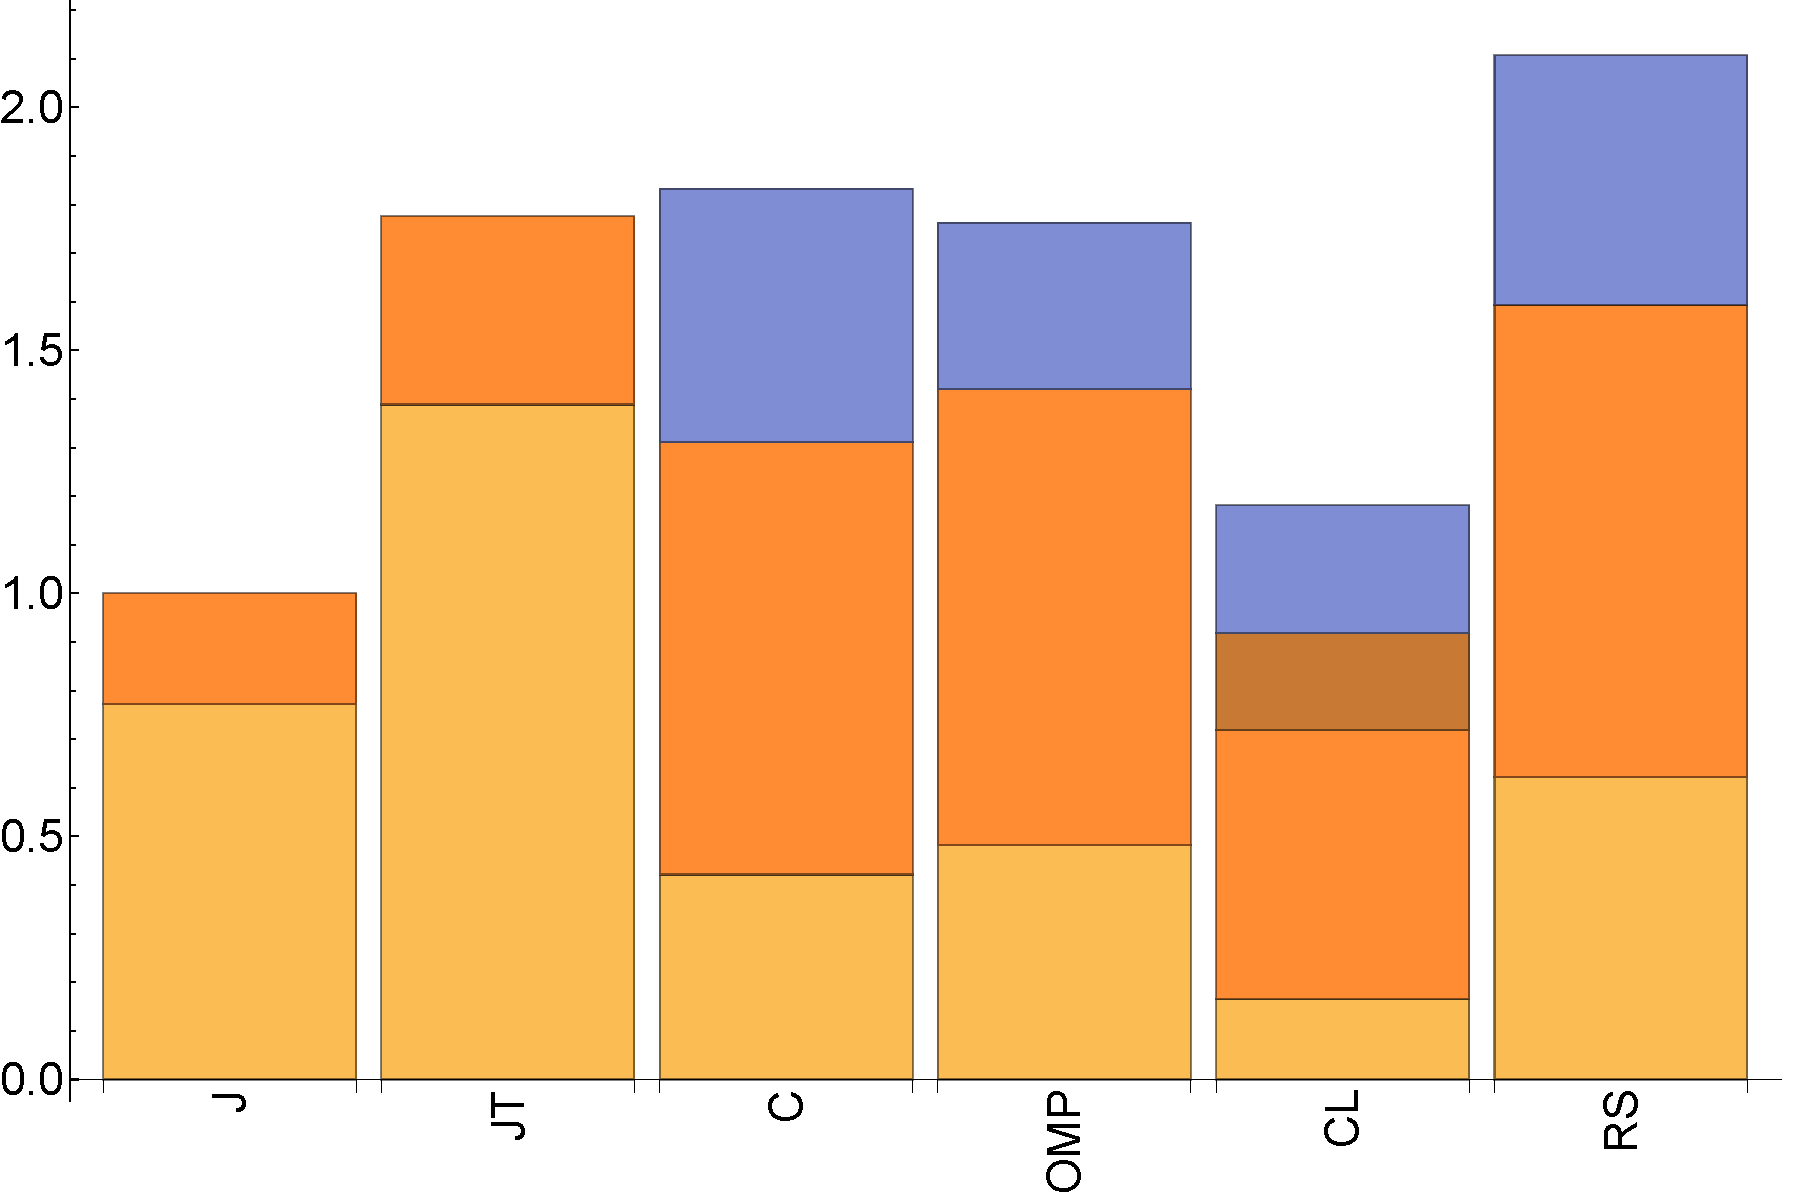
\includegraphics[width=\textwidth]{data/bbattery_vectoradd_nexus5.pdf}
      \caption{VectorAdd}\label{fig:vectoradd}
  \end{subfigure}
  \begin{subfigure}[b]{0.5\textwidth}
      \centering
      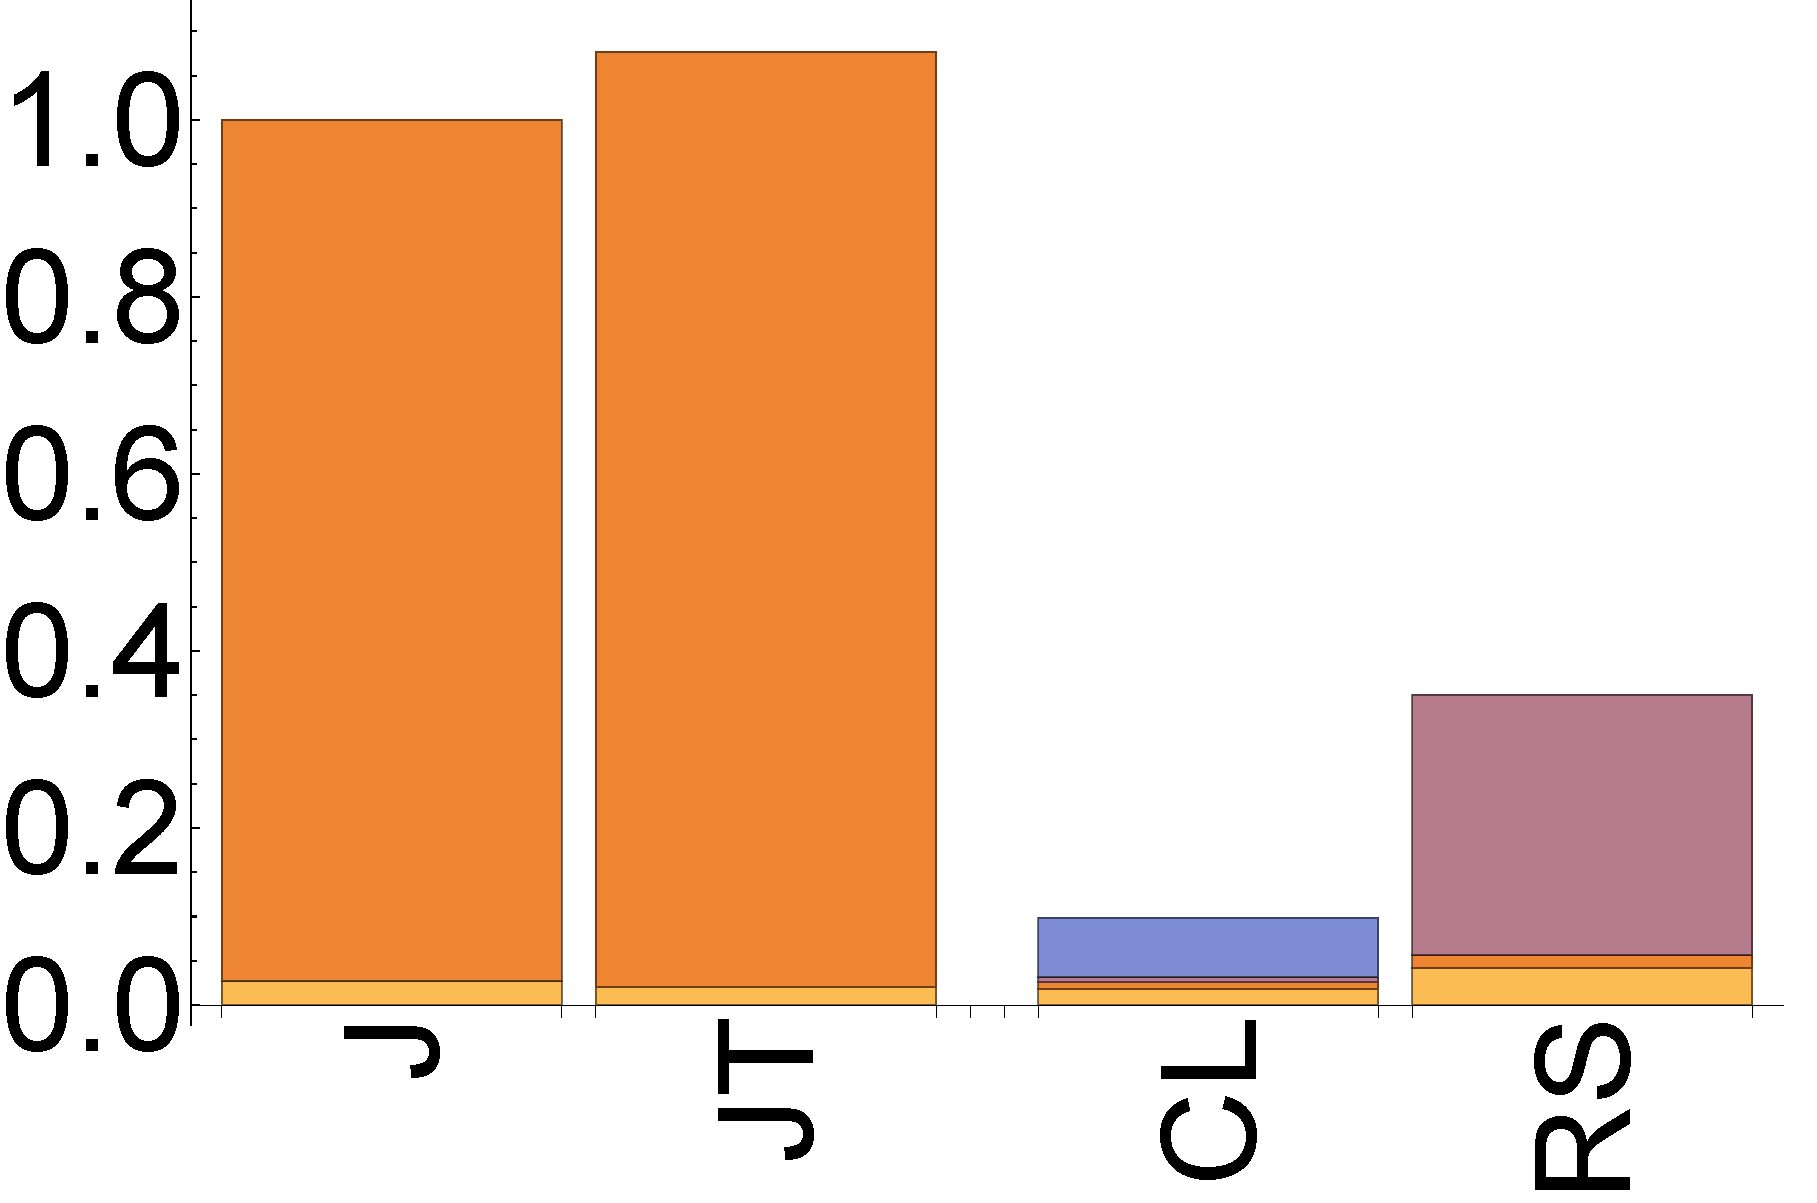
\includegraphics[width=\textwidth]{data/bbattery_tpacf_nexus5.pdf}
      \caption{TPACF}
      \label{fig:TPACF}
  \end{subfigure}

  \begin{subfigure}[b]{0.5\textwidth}
      \centering
      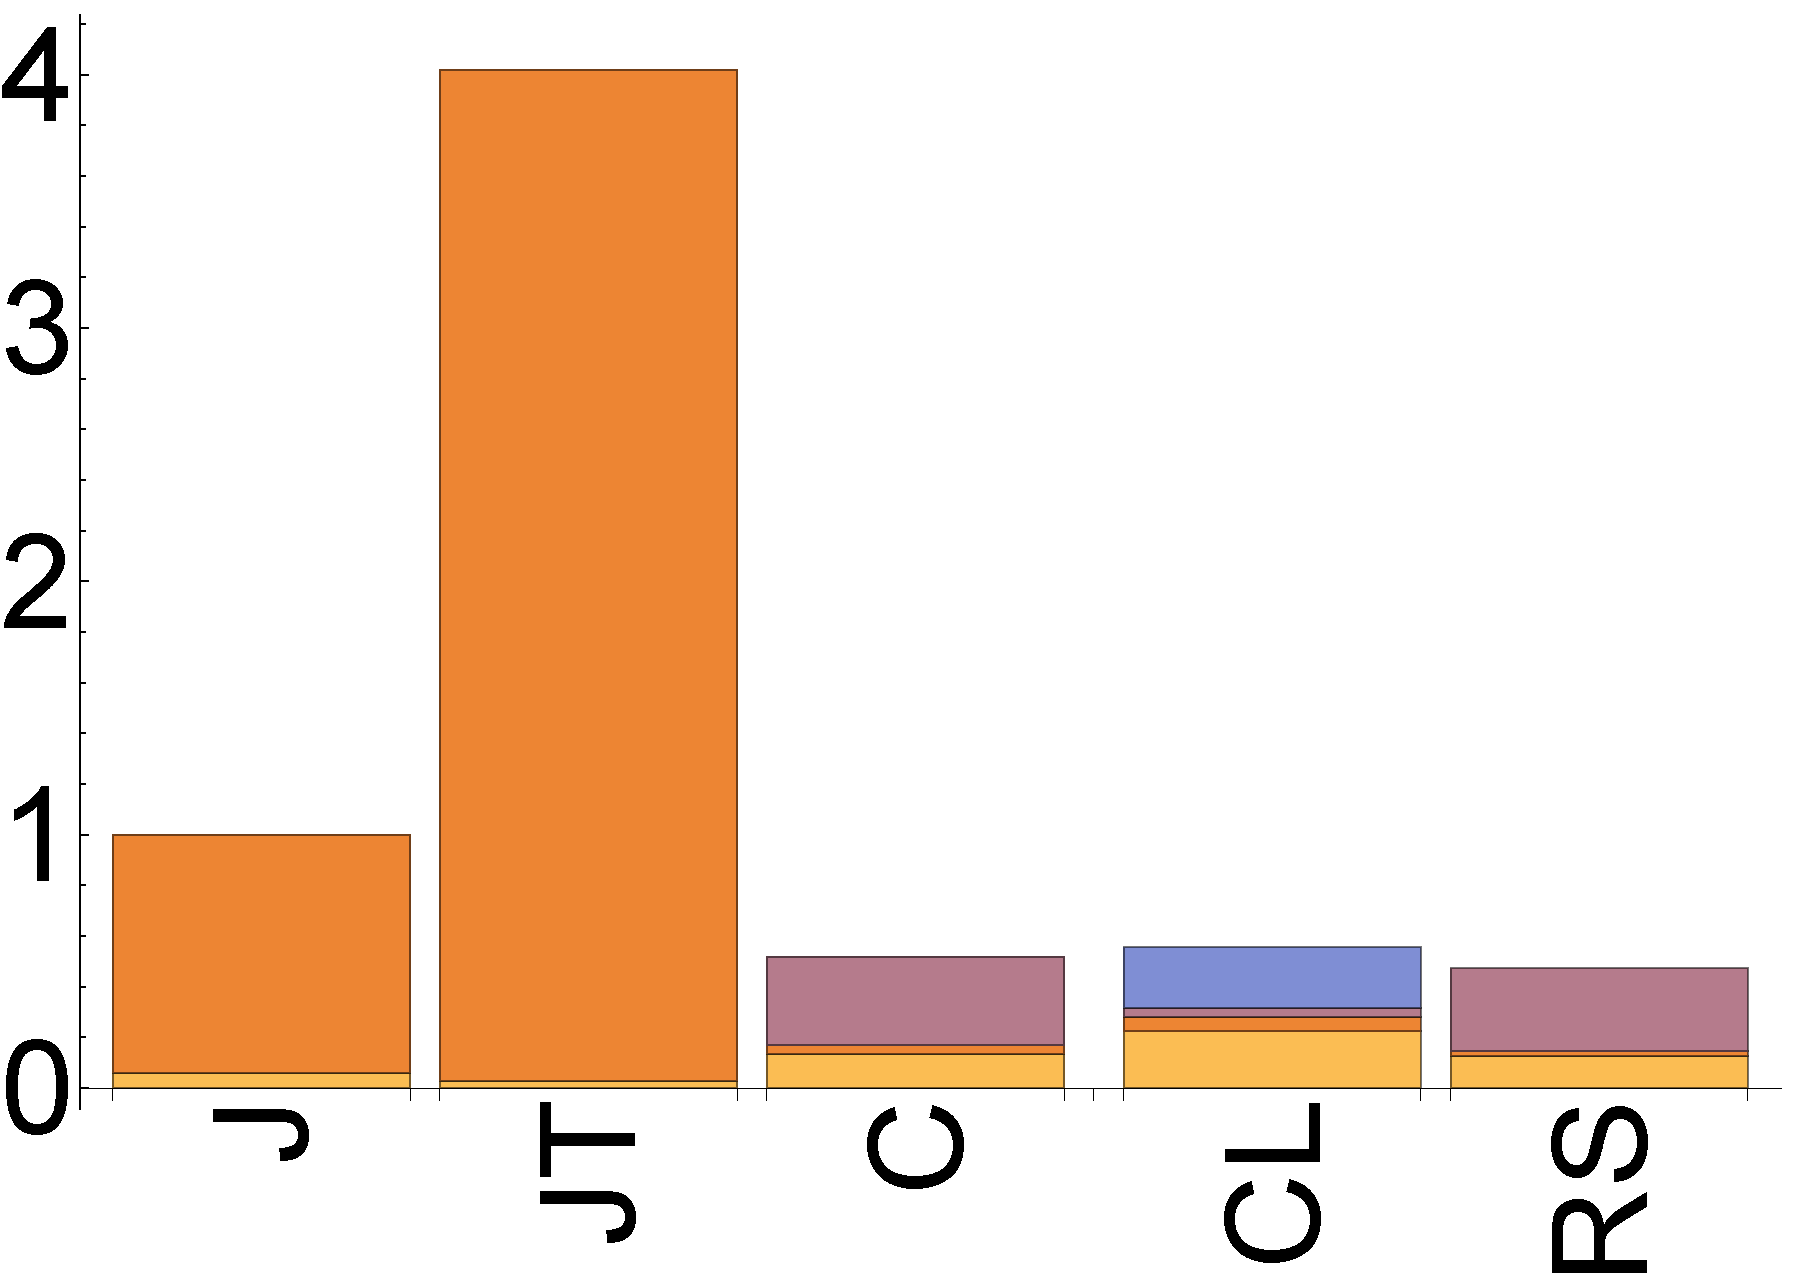
\includegraphics[width=\textwidth]{data/bbattery_histogram_nexus5.pdf}
      \caption{Histo}\label{fig:histo}
  \end{subfigure}

  \begin{subfigure}[b]{0.5\textwidth}
      \centering
      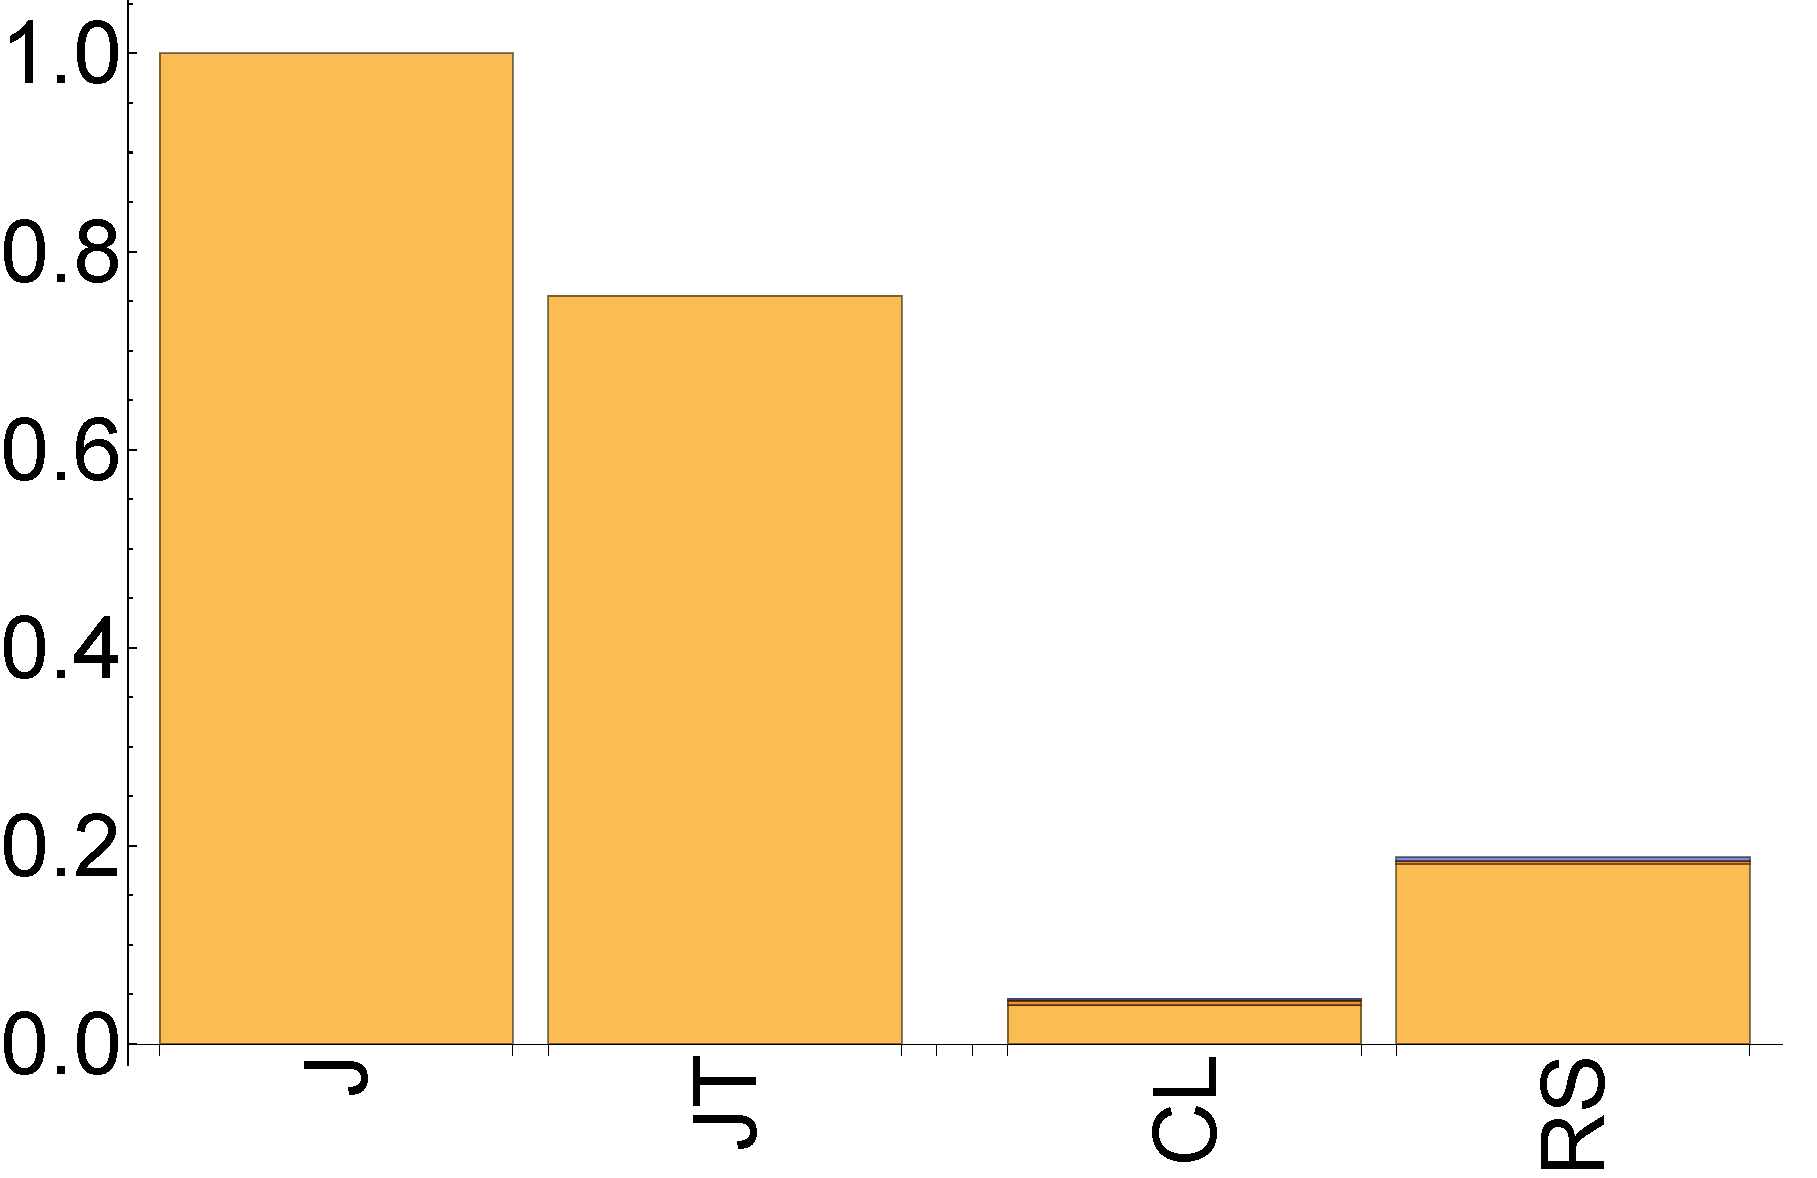
\includegraphics[width=\textwidth]{data/bbattery_mriq_nexus5.pdf}
      \caption{MRIQ}
      \label{fig:MRIQ}
  \end{subfigure}

  \begin{subfigure}[b]{0.5\textwidth}
      \centering
      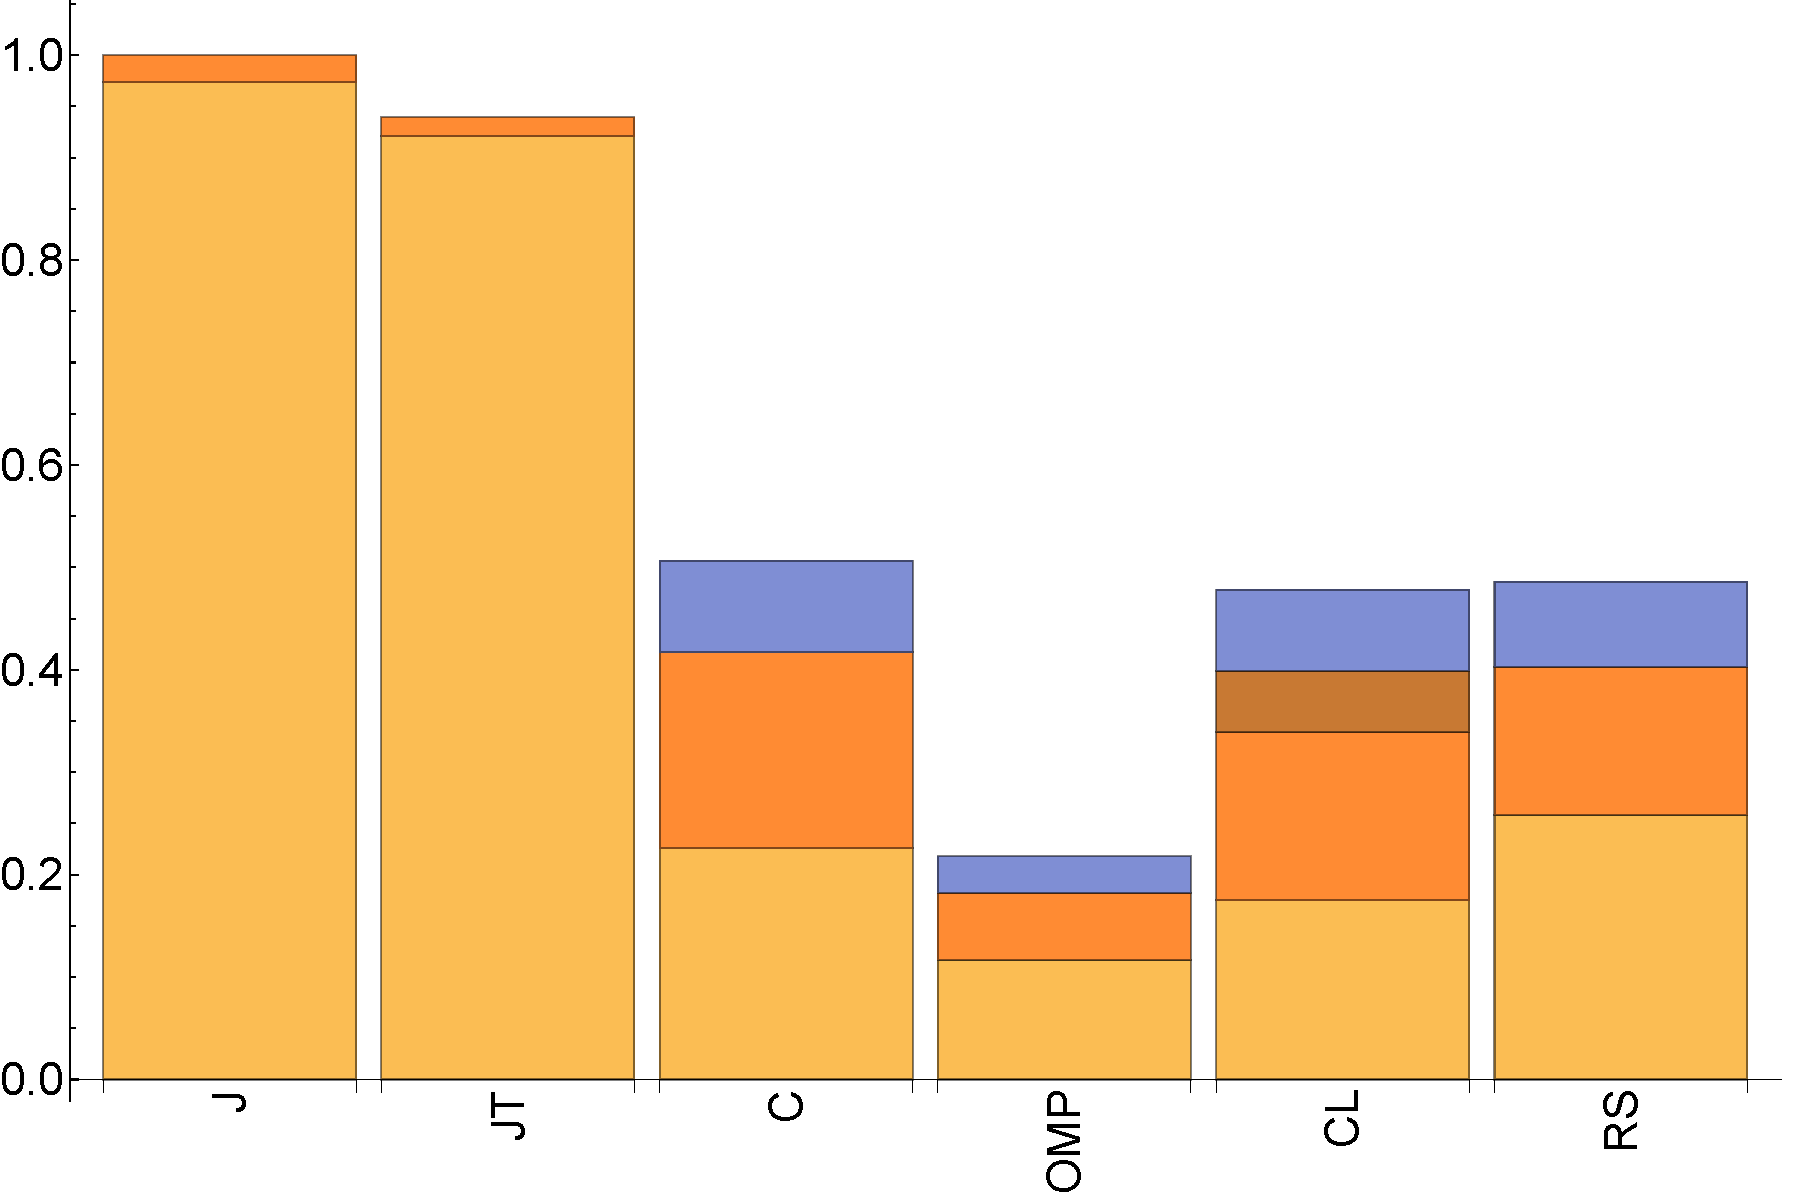
\includegraphics[width=\textwidth]{data/bbattery_sgemm_nexus5.pdf}
      \caption{Sgemm}\label{fig:Sgemm}
  \end{subfigure}
  \begin{subfigure}[b]{0.5\textwidth}
      \centering
      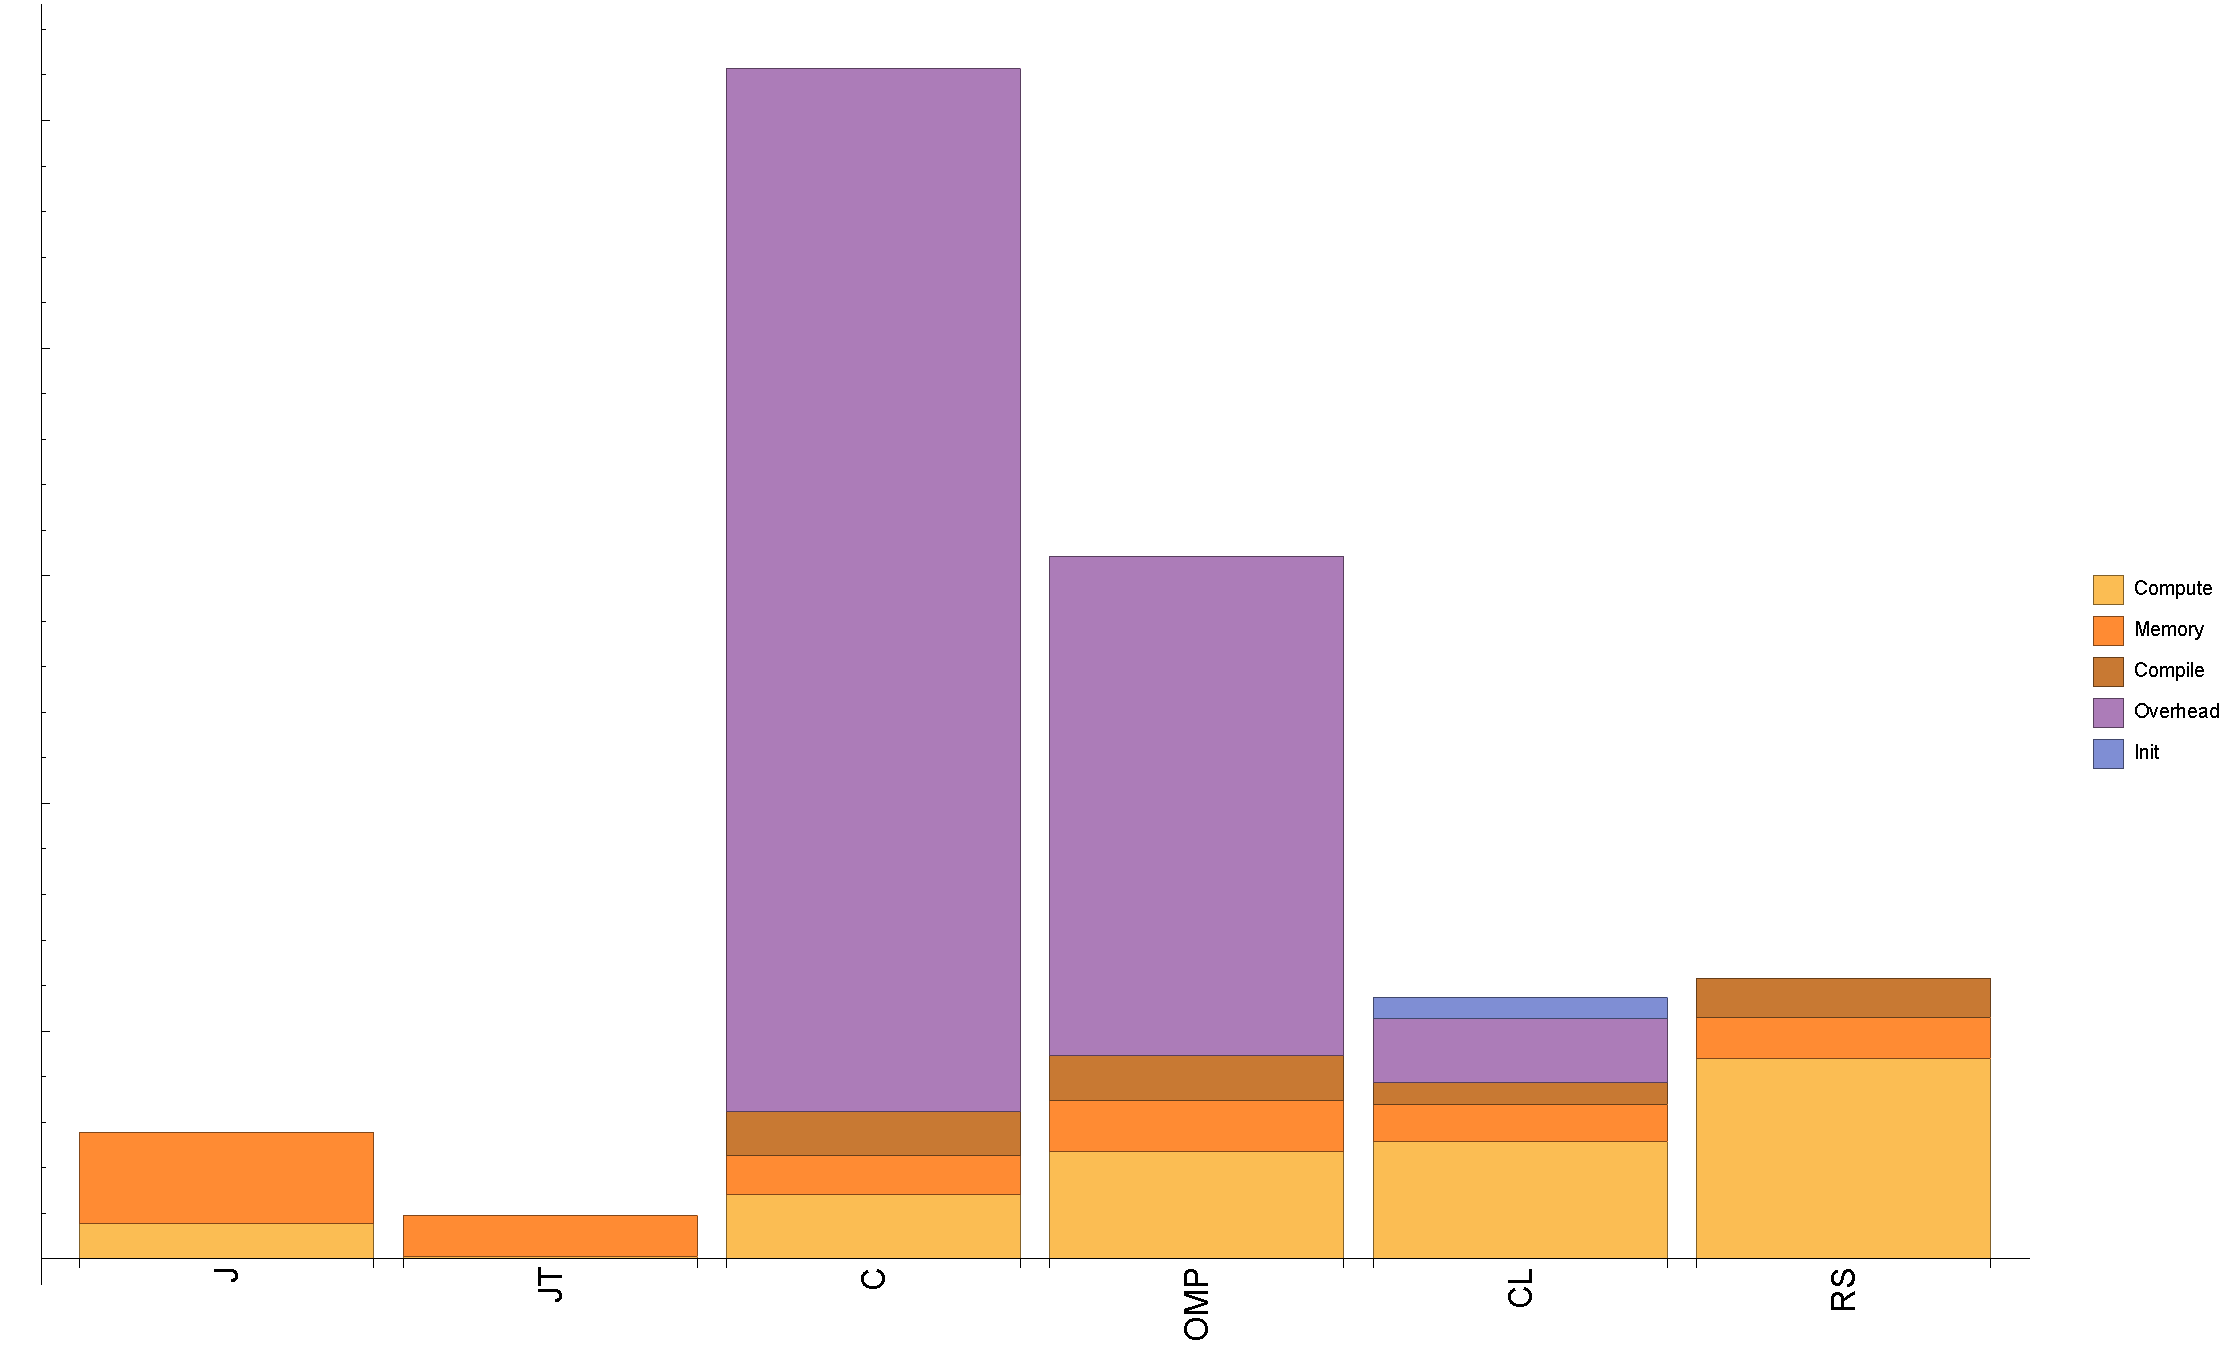
\includegraphics[width=\textwidth]{data/bbattery_stencil_nexus5.pdf}
      \caption{Stencil}
      \label{fig:Stencil}
  \end{subfigure}

  \caption{Battery Nexus 5}
\end{figure*}

Note: Battery information consists of all power-consuming components, e.g., screen,
cpu, gpu, memory. If the computation takes longer, more battery power has to
be spent on other components, such as screen, which typically consumes more
power than the cpus or gpus. That why we think the results that we got
reflects the actual power consumption in real usage of mobile devices.

\subsubsection{Vector Add}

\subsubsection{SGEMM}

\subsubsection{Stencil}

\subsubsection{Histogram}

\subsubsection{CUTCP}
